\chapter{Static code analysis}
Detecting errors in code early in development process is important to reduce cost of repairing such errors. The most commonly used process to detect errors as soon as possible is called \emph{code review}. Static code analysis can be considered to be automated code review.

One of the biggest pitfalls of code review is its high price, when big portion of development budget consists of developer salaries. Two or more people read code looking for a way to improve it, finding and fixing errors or potential errors that can become real errors in future, performance issues, etc. Quality of code review also decreases with time spent reading code. Developers need to rest to increase quality of a review.

Compiler warnings can be considered to be very basic static code analysis performed by compiler. It warns programmer about suspicious parts of code it detected in compilation process. It is good practice to turn on all warnings in compiler and compile code without any detected. The most commonly used compilers also provides switch to consider warnings as an errors. Software development companies often create rules to force programmers produce warning-less code or simply using mentioned compiler switch in development environment to implicitly remove warnings.

But there's not much compilers can do in diagnosing more complex errors. It's not their primary goal which is code compilation and more advanced diagnostic could hurt compilation times. In context of this thesis, where C++  is the analysed language, compilation times do really matter. Furthermore, there's no need to produce any binary when analysing code. Developer of tool for static code analysis would like to step in right after semantic analysis finished when there's enough understanding of source code. It's up to programmer whether he reuses front-end of compiler or implements his own.

\section{Pitfalls}
Due to complexity of C++ core language, there are only a very few fully C++ compliant, open-source and freeware\footnote{Proprietary compilers could do the job as well, but freeware compilers are preferred ones.} compilers. The two most known are \emph{GCC, the GNU Compiler Collection} and \emph{Clang/LLVM}. Apart from standard syntax for procedural programming, C++ standard includes Turing-complete template metaprogramming language. Simplified, compiler needs to \textit{"execute"} code to generate code that will be eventually compiled into native code. As an example of language complexity, implementation of \code{export} feature, which allows programmers to define template code in one translation unit and use in different, was so huge task for compiler vendors\footnote{Only one compiler vendor was able to implement it, \emph{Comeau C/C++}.} that this feature was eventually removed from language\footnote{Keyword has remained in language for future purpose.}. Based on given facts, it would be extremely difficult and unwise to individually implement own C++ front-end.

This chapter will cover some of the possible approaches for creating static code analysis tool apart from using Clang. It is covered by the next chapter.

\section{GCC - the GNU Compiler Collection}
GCC is compiler with great and 26 year old history and is well established in C++ software development world. A lot of helper tools for build environment support GCC in some way and yet, as it was already mentioned, programmers were struggling with writing static code analysis tools for C++. Why not just use GCC? Cite from Sparse FAQ [link] partially covers the answer:\\

\emph{"Gcc is big, complex, and the gcc maintainers are not interested in other uses of the gcc front-end.  In fact, gcc has explicitly resisted splitting up the front and back ends and having some common intermediate language because of religious license issues - you can have multiple front ends and back ends, but they all have to be part of gcc and licensed under the GPL."}\\

The first sentence, especially the first few words, is the main reason programmers haven't started using GCC front-end to create tools for static code analysis.

Brief list of cons:

\begin{itemize}
\item It's very hard to learn for beginners.

\item Even though GCC consists of front-end, middle-end and back-end, it \textit{"feels"} monolithic by design. It's very difficult to decouple front and back ends.

\item GENERIC and GIMPLE\footnote{Names for different representations of AST. GIMPLE is subset of GENERIC for code optimizations.} representations of code are not intuitive.

\item GCC doesn't keep track of tokens location in source code, e.g., it doesn't keep track of macro expansions so it's very difficult to correctly refactor code.

\item Code is optimized when it is parsed. Therefore AST doesn't correspond to source code, e.g., \code{x-x} is optimized to be \code{0}. It's extremely difficult to refactor code based on such optimized AST.
\end{itemize}

Subjective con:

\begin{itemize}
\item Code base is written mainly in C language. Even though there's ongoing transition to C++, it's not going to change design of the compiler. Transition will introduce only a very few and simple C++ features, e.g., STL containers such as \code{std::vector}, smart pointers to partially replace GCC internal garbage collection, templates, etc.
\end{itemize}

\section{Elsa: The Elkhound-based C/C++ Parser}
Even a smaller group of developers is able to create relatively nice C++ compiler front-end. Elsa is such an example. It provides programmer with user friendly AST representation of code, which is designed in the way it is easily extensible without writing single line of C++ code. For AST traversal, front-end provides mechanism designed as \emph{Visitor pattern}. The other way is to manually traverse tree by following edges. Visitor pattern is useful for context insensitive traversal. Within chapter dedicated to Clang, reader will discover that both approaches are very similar to what Clang provides developer.

The biggest disadvantage of Elsa is that its development stopped long time ago in 2005 when different project, called \emph{Oink}, which uses Elsa front-end started. Oink development then stopped before year 2011 when C++ experienced its \textit{"renaissance"} with the new approved standard since 2003, which introduced big changes to core language and library. Therefore there's almost no support for new C++11 language features. Oink as well as Elsa doesn't have integrated preprocessor and so it's extremely difficult to map AST with locations in source code. Elsa also suffers from lower speed, but for small projects it may be negligible.

\section{VivaCore/OpenC++}
Library was created as basis for \emph{PVS-Studio} static code analyser for C/C++ code. VivaCore is derived from older \emph{OpenC++ (OpenCxx)} library. The idea of using OpenC++ appeared when team was implementing \emph{Viva64} library. They've made a lot of changes to OpenC++ and because lack of resources they didn't continue to improve it\footnote{Many changes didn't fit into OpenC++ ideology so they would need to adapt and allocate new resources for such process.}, but rather developed their own library. Library became popular and is used as basis by other very popular tools such as  \emph{VisualAssist} by \emph{Whole Tomato Software}, \emph{Doxygen}, \emph{Gimpel Software PC-Lint}, \emph{Parasoft C++test} and more.

\begin{figure}[h!]
\label{vivacore}
\caption{Data flow graph in VivaCore library.}
\centering
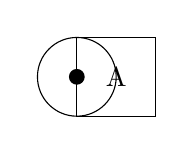
\begin{tikzpicture}[node distance=.5cm]
% \node[punkt](preprocessor) {External preprocessor};
% \node[punkt, below=of preprocessor](internal) {Preprocessor subsystem};
% \node[punkt, below=of internal](lexer) {Lexer};
% \node[punkt, below=of lexer](parser) {Parser};
% \node[punkt, below=of parser](walker) {PT Walker};
% \node[punkt, below=of walker](metaprogram) {Metaprogram subsystem};

	\node[matrix] (A) {
        \draw (0,0) rectangle (1,1); 
        \node at (0.5,0.5) {A}; \\
    };
    \node[matrix,left of=A] (B) 
    {
        \draw (0.5,0.5) circle (0.5);
        \fill (0.5,0.5) circle (0.1); \\
    }; 
 
\end{tikzpicture}
\end{figure}

The first step of code analysis is to use preprocessor. Library uses external preprocessor what becomes its biggest disadvantage in source-to-source transformation process. Without integrated preprocessor it's next to impossible to track macro expansion and actual location of symbols in source code. Doxygen users should now understand why there's special \code{\textbackslash{def}} command to define macro documentation since it doesn't see macro definition and usage because of using external preprocessor and seeing only preprocessed code.

Preprocessed input is then passed to library. There are two library subsystems that process code before it gets to lexical analysis. The first is input subsystem which has responsibility for putting preprocessed code into internal data structures. The second step is internally called \emph{Preprocessor}, but it doesn't preprocess input in the meaning of C++ preprocessor. It has mainly responsibility for two operations:

\begin{itemize}
\item Splitting code into strings and dividing them into two logical groups. One is for system libraries and the second one is for user code. Library user can choose whether he wants to analyse system code or just user code.
\item Removing C++ non-related strings, specific for compiler, e.g., \code{SA\_Success} and \code{SA\_FormatString} are presented in Visual Studio headers.
\end{itemize}

Next step is lexical analysis. Output of \emph{Lexer} can be used for basic metrics or syntax highlighting. VivaCore allows to easily modify set of tokens for lexical analysis.

VivaCore provides user with \emph{parse tree (PT)} called also \emph{derivation tree (DT)} as an output of syntactic analysis. Parse tree differs from abstract syntax tree in the way it contains nodes representing derivation rules used in syntactic analysis. The word \emph{abstract} came from the reasoning that it hides the way tree was constructed. It is actually possible to traverse PT as it was AST. VivaCore`s PT defines two basic sets of nodes with ancestors in \code{NonLeaf} and \code{Leaf} base classes which have \code{PTree}\footnote{\code{PTree} has \code{LightObject} as its base class used in GC.} class as their common ancestor declaring the only pure virtual member function:

\begin{lstlisting}
virtual bool IsLeaf() const = 0;
\end{lstlisting}

It is actually the only function that is needed to be defined in inherited classes letting their design to be more flexible.

Probably the most interesting part of library interface is tree traversal. There are three different \emph{walker} classes implemented for this purpose.

\begin{description}
\item[Walker] is responsible for walking over basic C++ constructions.
\item[ClassWalker] handles C++ class specific features.
\item[ClassBodyWalker] traverses body of C++ class.
\end{description}

It is possible to traverse PT multiple times so user can traverse code for measurements at first and later, in further traversals, he may modify PT. If user modifies tree nodes, it may occur that tree is rebuilt.

\section{Related work}
Code quality in a huge projects is hard to maintain using code review since there's a lot of code related commits every day (e.g. Crysis 2 multiplayer had $\sim$100-150 code related commits every day collecting 103 different developers in its lifetime) and providing people resources for code review would be inefficient. Instead of that, companies use tools for static code analysis and diagnostic is further reviewed. Though not many companies trust tools in the way they let them do source-to-source transformations apart from formatting or simple refactoring.

\subsection{Clang Static Analyzer (\emph{clang-analyzer})}
\label{clanganalyzer}
Static analyser is part of the Clang project implemented on top of Clang tooling API. Analyser is quite easily expandable by implementing \emph{checkers}, even though their interface may not be intuitive. Authors created presentation where they try to explain \emph{"How To Write a Checker in 24 Hours"}[link]. They demonstrate how to write simple checker for  Unix stream API. When writing checker, developer needs to understand how analyzer works under the hood.

Core of the analyser does symbolic execution of code, exploring every possible path, tracking all variables and constructing \emph{Control Flow Graph (CFG)}. Checkers participate in CFG construction. Essentially, checkers are visitors that react on specific set of events while traversing AST (e.g. \code{checkPreStmt}, \code{checkPostCall} functions) and eventually creating new CFG nodes. When they want to finish CFG exploration, they create \emph{sink} node. Checkers are stateless (i.e. visitor related member functions are defined as \code{const}) keeping their "state" data in \code{ProgramState} and its \emph{Generic Data Map (GDM)}.

Previous paragraphs describes analyser and checkers very briefly and from given information and without an example it's hard to understand how checkers are exactly supposed to be implemented. On the other hand, mentioning CFG should give reader basic idea of what code problems analyser aims to check. It's not that hard to check bad usage patterns in code using Clang tooling facilities such as AST visitor and matchers. The way harder problems are problems related to resource acquisition and release such as resource leaks or resource usage after release. The development manual page of analyser contains very good advice for implementation of checkers[link]:\\

\label{clang-analyzer-checkers}
\emph{"Some checks might not require path-sensitivity to be effective. Simple AST walk might be sufficient. If that is the case, consider implementing a Clang compiler warning. On the other hand, a check might not be acceptable as a compiler warning; for example, because of a relatively high false positive rate."}

\subsection{Clang Format (\emph{clang-format})}
\label{clang-format}
Consistency in code formatting is very important in huge projects. It increases readability and code also becomes better machine editable. Even though consistent code formatting is very important, there's not a lot of tools that support automatic code formatting for C++ (e.g. \textit{BCPP}, \textit{Artistic Style}, \textit{Uncrustify}, \textit{GreatCode}, \emph{Style Revisor})

The reason why companies allow use of an automatic formatting tools is that those tools guarantee they won't change code semantic (i.e. they edit only white space characters, literals and comments) and thus won't break compilation. In this context, there was proposal to let clang-format reorder includes, but it wasn't approved, because such change can break compilation. Main challenges for clang-format based on their design document [link]:

\begin{itemize}
\item A vast number of different coding styles has evolved over time.
\item Macros need to be handled properly.
\item It should be possible to format code that is not yet syntactically correct.
\end{itemize}

It was a hard decision for clang-format authors whether they use Lexer or Parser to implement such tool. Both have their advantages and disadvantages in terms of performance, macro management, type info, etc. In the end they decided to stick with implementation based on Lexer, but there's still a discussion about adding AST information. Though this discussion is leaning towards creating separate tool using AST, which already has the name, \emph{clang-tidy}.

\subsection{OCLint}
Another tool built on top of Clang LibTooling interface is \emph{OCLint}. Main parts of OCLint are \emph{Core}, \emph{Rules} and \emph{Reporter}.

Core controls the flow of analysis, dispatches tasks to another modules and outputs results. It parses code creating AST and provides modules with access to it. While parsing code it creates various metrics such as:

\begin{itemize}
\item Cyclomatic complexity.
\item NPath complexity.
\item Non commenting source statements.
\item Statement depth.
\end{itemize}

\emph{Rules} may then provide \emph{RuleConfiguration} that defines limits for metrics. When limits  are exceeded, \emph{Core} emits violation. There are two main approaches for modules to handle diagnostic:

\begin{description}
\item[Line based] is when modules are provided with lines of code.
\item[AST based] provides modules AST access using another two approaches  \footnote{Without further details. Very similar mechanisms will be mentioned in the following Clang chapter.}:
	\begin{itemize}
	\item Using \emph{Visitor pattern} to explore AST.
	\item Defining \emph{Matchers} for suspicious code patterns.
	\end{itemize}
\end{description}

Actually, OCLint tries to create generic framework for code diagnostic. Modules are separated from \emph{Core} code and can be loaded in runtime. Basic diagnostic can be really represented as set of code \textit{"bad usage"} patterns, where AST matchers become very comfortable mechanism. Reporting found \textit{"bad usage"} is the last task to be done.

From the negative side, pattern matching is not strong enough mechanism to catch even a little more complex errors such as resource leak. The other supported approaches than AST matchers don't really help more then just using Clang tooling API. It would be nice to remind advice from clang-analyzer developer manual (see Section \ref{clang-analyzer-checkers}).

\subsection{Scout}
\label{scout}
The first, unfortunately also the last, tool that does also source-to-source transformations what create another dimension of problems regarding static code analysis. Scout is being developed in \emph{TU Dresden}, \emph{Center for Information Services and High Performance Computing}. It is supposed to do transformations for front-end SIMD optimizations (e.g. loop vectorization), very similar task to what the most current compiler back-end optimizers do. It shall transform C code into optimized C code with compiler intrinsics. Naturally, auto-vectorization is done by compiler back-end optimizer, but there are limits to what compiler can do. It needs to use extensive dependency and alias analysis to reason correctness of vectorization and often rejects more complex loops. Some compilers allow programmers to annotate loops with \code{pragma} directives giving responsibility for keeping some loop invariants to programmers. Compiler can skip those checks before vectorization thus accepting more loops. Unfortunately, the measurement with specific Intel compiler using \code{pragma} directives gave insufficient results. For example compiler rejected loop vectorization after loop variable was changed from \code{unsigned int} to \code{signed int}. Actually, Scout provides semi-automatic vectorization, where programmers need to annotate loops using \code{pragma} directives to enable vectorization of given loop. 

Tool provides command line interface as well as graphical user interface. It is built over the Clang parser to build AST from C code. AST is then transformed to different AST that represents optimized code and transformed back to C code. Scout is implemented in the way it can be used in a built process. Tool can be configured with set of intrinsics to be used (i.e. \emph{SSE2}, \emph{SSE4}, \emph{AVX}, \emph{AVX2} or \emph{ARM NEON}).

\subsubsection{Source-to-source transformation}
Possibilities of source-to-source transformations using Clang API will be described in more details in the following chapter dedicated to Clang. Scout authors chose to directly edit AST, approach that is not recommended by the Clang developers. It is work in progress to use \code{TreeTransform} facility, probably the only correct approach, but with lower priority because \textit{"it just works"} with AST manipulation for now.

The central class for AST editing is called \code{StmtEditor}. Is is supposed to ease creation of new nodes and putting them together. What Clang provides is actually much more than just AST so node creation and insertion are complex operations which are supposed to be covered by this class. Scout implements them in naive way when there can exist usages that will create semantically invalid AST. As far as user knows how these member functions can be used, it should be fine to modify AST. Programmer is supposed to inherit from \code{StmtEditor} class and use its member functions to manipulate with AST. After AST transformations are done, it should be passed back for semantic analysis. Currently in Scout, it is not.

\subsection{Cppcheck}
The first tool in the list which doesn't use any compiler front-end as helper for parsing C++ code. CppCheck does code parsing and analysis on its own, but with lower quality of understanding of code than well established compiler front-ends. Input for checks is output of lexical analysis and it may be very difficult to implement more advanced checks. The fact that code analysis passes only lexical analysis phase does also mean that tool is not able to catch even syntactic errors. To ease programmers life, CppCheck implements classes such as \code{Scope} or \code{SymbolDatabase} with functionality the names indicate.

Simplified version of CppCheck execution from programmers documentation[link]:

\begin{enumerate}
\item Parse command line.
\item \code{ThreadExecutor} creates needed \code{CppCheck} instances.
\item \code{CppCheck::check} is called for every file.
\item Inside \code{check}, preprocess file.
    \begin{itemize}
    \item Comments are removed.
    \item Macros are expanded.
    \end{itemize}
\item Tokenize file using \code{Tokenizer}.
\item Run all checks on tokenizer output called token list.
\item Simplify token list.\footnote{There are various simplifications applied to token list. Every simplification passes the whole token list looking for patterns and potentially changes this list. For example the first applied simplification changes \code{"string"[0]} to \code{'s'}. Another example is removing \code{std::} tokens from specific set of function calls.}
\item Run all checks on simplified token list.
\end{enumerate}
